\documentclass[a4paper,10pt]{article}
\usepackage[utf8]{inputenc}
\usepackage{graphicx}
\usepackage{amsmath}
\usepackage{geometry}
\usepackage{multicol}
\usepackage{fancyhdr}
\usepackage{titlesec}
\usepackage{parskip}
\usepackage{tabularx}
\usepackage{multirow}
\usepackage[table,xcdraw]{xcolor}
\usepackage{colortbl}
\usepackage{caption}
\usepackage{subcaption}
\usepackage{adjustbox}
\usepackage{siunitx}
\usepackage[version=4]{mhchem}
\usepackage{wrapfig}
\DeclareSIUnit\molar{M}
\DeclareSIUnit\angstrom{\text{\AA}}

\geometry{left=1in, right=1in, top=1in, bottom=1in}

\titleformat{\section}{\normalfont\large\bfseries}{\thesection}{1em}{}
\titleformat{\subsection}{\normalfont\normalsize\bfseries}{\thesubsection}{1em}{}


\titlespacing*{\section}{0pt}{1.5ex}{0.8ex}
\titlespacing*{\subsection}{0pt}{1.2ex}{0.6ex}



\pagestyle{fancy}
\fancyhf{}
\fancyfoot[C]{\thepage}
\fancyhead[L]{Projeto em Engenharia Aeroespacial}
\fancyhead[R]{Ano letivo 2025/26}

\begin{document}

{\Large\textbf{\parbox[t]{\textwidth}{\centering Corrosion protection of complex shapes aluminium alloys via conversion coatings}}}
\vspace*{12pt}
\begin{tabularx}{\textwidth}{X}
Alexandre de Brito Salvador Cauvel \\
\texttt{alexandre.cauvel@ua.pt} \\
\textit{Advisors: Kiryl Yasakau, João Tedim}
\end{tabularx}
\vspace{12pt}
\hrulefill

\begin{abstract}
This work investigates the development of a ZnAl--LDH conversion coating system loaded with corrosion inhibitors on the AC46000 die-cast aluminium alloy as a chromate-free alternative for aerospace applications. Electrochemical pre-selection identified MBT, \ce{NaVO3}, and L-cysteine as the most effective inhibitors. While \ce{NaVO3} was successfully intercalated into the LDH galleries, demonstrating active chloride-triggered release, the thiol-containing inhibitors caused the complete dissolution of the LDH structure due to aggressive zinc chelation. Corrosion evaluation highlighted the critical influence of the substrate microstructure: an aggressive industrial pre-treatment proved detrimental by exposing subsurface intermetallics during LDH synthesis. A milder chemical pre-treatment yielded significant improvements, with MBT providing excellent initial barrier protection and \ce{NaVO3} providing sustained active protection. Potentiodynamic polarisation confirmed both act primarily as anodic inhibitors, though neither effectively suppressed cathodic activity at Fe--Mn intermetallic sites. Finally, the successful application of a polyurethane topcoat via anodic electrodeposition on complex geometries validated the practical feasibility of the complete multilayer system.
\end{abstract}
\hrulefill

\begin{multicols}{2}


\section{Introduction}
Modern aerospace structures rely heavily on high-performance aluminium alloys, particularly the 2xxx and 7xxx series, due to their exceptional strength-to-weight ratio. However, in harsh aerospace environments, these materials are highly susceptible to localised corrosion, accelerated by dispersed intermetallic particles (IMPs) that form micro-galvanic sites \cite{MartinezViademonte2020, Garg2025}. Traditionally, this challenge has been managed using multilayer coatings based on hexavalent chromium (Cr(VI)), which offer exceptional self-healing capabilities. However, the carcinogenic nature of Cr(VI) has led to strict regulatory restrictions, creating an urgent need for high-performance, environmentally benign alternatives \cite{Becker2019, BoualiReview2020}.

Layered Double Hydroxides (LDH) have emerged as a highly promising chromate-free alternative. Their unique layered structure allows for the storage and stimuli-responsive release of corrosion inhibitors via anion exchange, providing a combination of barrier protection and active self-healing \cite{Cao2022, Yasakau2018, Zhou2017}. While recent LDH research has demonstrated excellent potential on wrought alloys (e.g., AA2024) tested on simple flat specimens \cite{Tedim2014, Tedim2011, He2020}, there is a distinct lack of data regarding their performance on cast alloys like AC46000. Cast alloys enable the manufacturing of complex, highly detailed geometries increasingly common in modern aerospace assemblies. However, they introduce significant challenges, including heterogeneous microstructures, higher silicon content, and complex surface topographies, all of which critically influence LDH growth and coating integrity.

The primary objective of this work is to synthesise and optimise a ZnAl--LDH conversion pre-treatment capable of forming a uniform coating on both flat and complex-geometry AC46000 substrates. This involves the intercalation of selected corrosion inhibitors, rigorous electrochemical evaluation, and the ultimate validation of the complete multilayer protective system, including an organic polyurethane topcoat, on industrially representative complex geometries.

\section{Methodology}
The experimental methodology was structured to systematically address the challenges posed by the AC46000 die-cast alloy microstructure. 

\subsection{Inhibitor Pre-selection}
Seven candidate inhibitors (\ce{NaVO3}, \ce{Na2MoO4}, MBT, BTA, 8-HQ, L-cysteine, and a blank NaCl control) were evaluated via Electrochemical Impedance Spectroscopy (EIS) over \qty{168}{\hour} of immersion in \qty{0.05}{\molar} NaCl. The charge-transfer resistance ($R_{\text{ct}}$) and double-layer capacitance ($C_{\text{dl}}$) were extracted using a custom automated fitting framework based on the Differential Evolution algorithm.

\subsection{Surface Pre-treatments and LDH Synthesis}
To mitigate the heterogeneous distribution of IMPs, three surface preparation routes were evaluated: mechanical polishing (reference), a simplified chemical pre-treatment, and an aggressive industrial pre-treatment. Following pre-treatment, ZnAl--LDH films were synthesised \textit{in situ} via a hot aqueous solution method at \qty{95}{\degreeCelsius} for either \qty{1}{\hour} (LDH-1) or \qty{3}{\hour} (LDH-2). The films were characterised using X-ray Diffraction (XRD) and Scanning Electron Microscopy with Energy-Dispersive X-ray Spectroscopy (SEM-EDS).

\subsection{Inhibitor Intercalation}
The top-performing inhibitors from the pre-selection phase were incorporated into the LDH galleries via anion exchange. \ce{NaVO3} was intercalated from a \qty{0.1}{\molar} solution. For the MBT, the solution pH was carefully adjusted with NaOH to deprotonate the thiol groups, imparting the net negative charge required for electrostatic uptake \cite{Tedim2010}.

\subsection{Corrosion Performance and Topcoat Application}
The active corrosion protection of the intercalated LDH coatings was evaluated via long-term EIS and Potentiodynamic Polarisation (PDP) in \qty{0.05}{\molar} NaCl \cite{Orazem2008}. Finally, a water-based polyurethane colloidal formulation was applied over the optimised LDH pre-treatments via anodic electrodeposition (\qty{80}{\volt} for \qty{1}{\minute}, followed by curing at \qty{120}{\degreeCelsius}) on both planar and complex-geometry specimens to form a complete multilayer system.

\section{Results and Discussion}

\subsection{Inhibitor Pre-selection}
The EIS pre-selection identified MBT, \ce{NaVO3}, and L-cysteine as the most effective inhibitors, demonstrating $R_{\text{ct}}$ values in excess of \qty{100}{\kilo\ohm} and stable $C_{\text{dl}}$ values on the order of \qty{10}{\micro\farad}, indicative of active and durable surface film formation. Sodium molybdate provided negligible protection. BTA and 8-HQ exhibited intermediate and transient protection, failing to maintain stable surface films over extended immersion.

\begin{center}
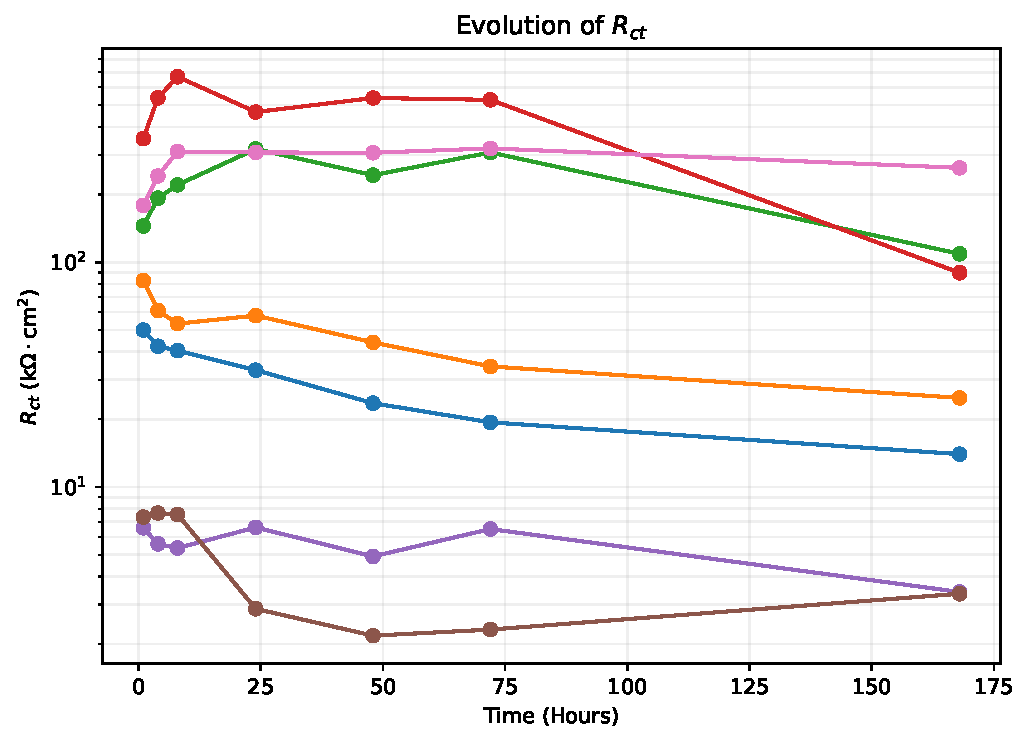
\includegraphics[width=0.9\linewidth]{Figures/Rct_evolution_inhibitors_resume.pdf}
\captionof{figure}{Evolution of $R_{\text{ct}}$ over the \qty{168}{\hour} immersion period for the pre-selected inhibitors.}
\label{fig:Rct_evolution_inhibitors}
\end{center}

% Figure 2: Cdl Evolution
\begin{center}
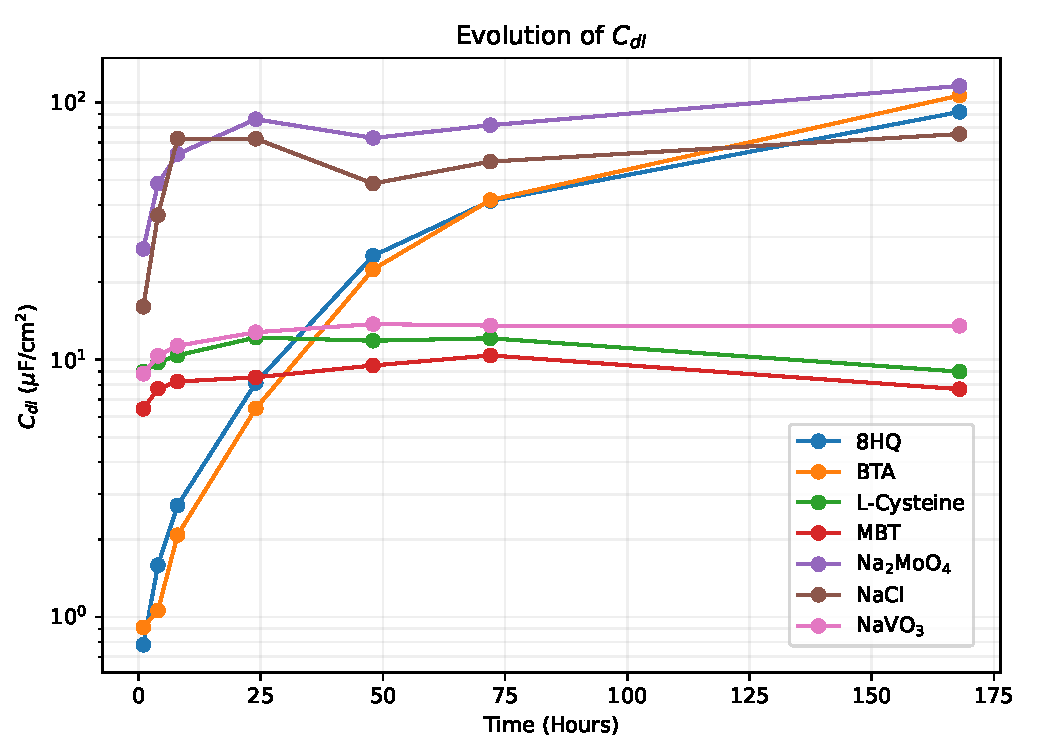
\includegraphics[width=0.9\linewidth]{Figures/Cdl_evolution_inhibitors_resume.pdf}
\captionof{figure}{Evolution of $C_{\text{dl}}$ over the \qty{168}{\hour} immersion period for the pre-selected inhibitors.}
\label{fig:Cdl_evolution_inhibitors}
\end{center}

\subsection{Pre-treatments and LDH Synthesis}
SEM-EDS characterisation revealed that the industrial pre-treatment achieved near-complete removal of Fe--Mn and Cu-rich IMPs, leaving primarily electrochemically inert Si particles exposed. The chemical pre-treatment achieved only partial removal of Fe--Mn particles. XRD analysis confirmed successful ZnAl--LDH formation on all substrate conditions, with comparable film density and basal spacing consistent with \ce{NO3-} intercalation. EDS analysis further confirmed uniform Zn deposition across both the aluminium matrix and the Si phase, demonstrating that the LDH grows conformally over the heterogeneous microstructure.

\subsection{Inhibitor Intercalation}
XRD analysis of the intercalated systems confirmed the successful incorporation of \ce{NaVO3}, evidenced by a systematic shift in the (003) basal reflection from $2\theta = 9.86^\circ$ to $9.51^\circ$, corresponding to an expansion of the interlayer gallery height from \qty{4.20}{\text{\AA}} to \qty{4.53}{\text{\AA}}. Following immersion in NaCl, a further shift to $2\theta = 10.35^\circ$ confirmed the exchange of vanadate for chloride anions, definitively demonstrating active inhibitor release \cite{Zhou2017}. 

In stark contrast, the attempted intercalation of MBT resulted in the complete dissolution of the LDH crystalline structure. This structural degradation is fundamentally attributed to the deprotonated, negatively charged thiolate anions (\ce{-S^-}) present in the alkaline intercalation solutions. These thiolate groups exhibit an exceptionally strong coordination affinity for \ce{Zn^{2+}} ions, acting as powerful chelating agents that actively extract zinc from the host brucite layers, forming soluble zinc--thiolate complexes and collapsing the LDH crystal lattice \cite{Tedim2010}. Consequently, this system lacks a structured reservoir for controlled release, restricting their protective mechanism to the passive barrier properties of the remnant amorphous oxide film combined with the direct chemisorption of MBT molecules onto the exposed alloy surface.


\end{multicols}

\begin{figure*}[!htbp]
    \centering
    
\includegraphics[width=0.8\textwidth]{Figures/XRD_intercalation.pdf} % Use \textwidth for full page width
    \caption{XRD patterns of LDH films in the nitrate form (control), following \ce{NaVO3} intercalation, and following the MBT intercalation attempt, each presented before and after immersion in 0.05 M NaCl.}
    \label{fig:xrd_intercalation}
\end{figure*}

\begin{multicols}{2}

\subsection{Corrosion Performance Analysis}
The corrosion performance was evaluated in two iterative batches. The first batch (LDH-1), based on the industrial pre-treatment with a \qty{1}{\hour} LDH growth time, yielded unsatisfactory protection. The uncoated control specimen outperformed all vanadate-intercalated LDH specimens. This counterintuitive result is attributed to the synergistic effect of the aggressive industrial etching and subsequent matrix dissolution: the etching digs deep trenches into the aluminium matrix, and even minor matrix dissolution during LDH synthesis fully exposes subsurface intermetallic particles that were previously undermined. These newly exposed, highly cathodic sites initiate severe localised pitting that the inhibitor loading is insufficient to suppress.

Driven by these limitations, the second batch (LDH-2) employed the milder chemical pre-treatment with an extended \qty{3}{\hour} LDH growth time. MBT-intercalated specimens exhibited the best corrosion protection, with a low-frequency impedance modulus approximately one order of magnitude higher than the control at \qty{1}{\hour} and substantially elevated $R_{\text{ct}}$ values at early immersion times. However, after \qty{24}{\hour}, their $R_{\text{ct}}$ values decreased sharply, confirming that the unstructured remnant film causes rapid inhibitor exhaustion via uncontrolled desorption and reprecipitation. \ce{NaVO3}-intercalated specimens showed intermediate performance, with localised vanadate oxide deposits confirming active inhibitor release and repassivation attempts. 

PDP analysis revealed that neither inhibitor suppressed cathodic activity at Fe--Mn sites, with cathodic branches virtually superimposed. However, both significantly reduced anodic dissolution, shifting $E_{\text{corr}}$ nobly and acting primarily as anodic inhibitors. The long-term performance remains below target due to persistent Fe--Mn particles on the chemically pre-treated surface. Unlike Cu-rich IMPs in wrought alloys like AA2024, the Fe--Mn IMPs characteristic of AC46000 are not effectively passivated by \ce{NaVO3} or MBT.

% Figure 1: Rct Evolution
\begin{center}
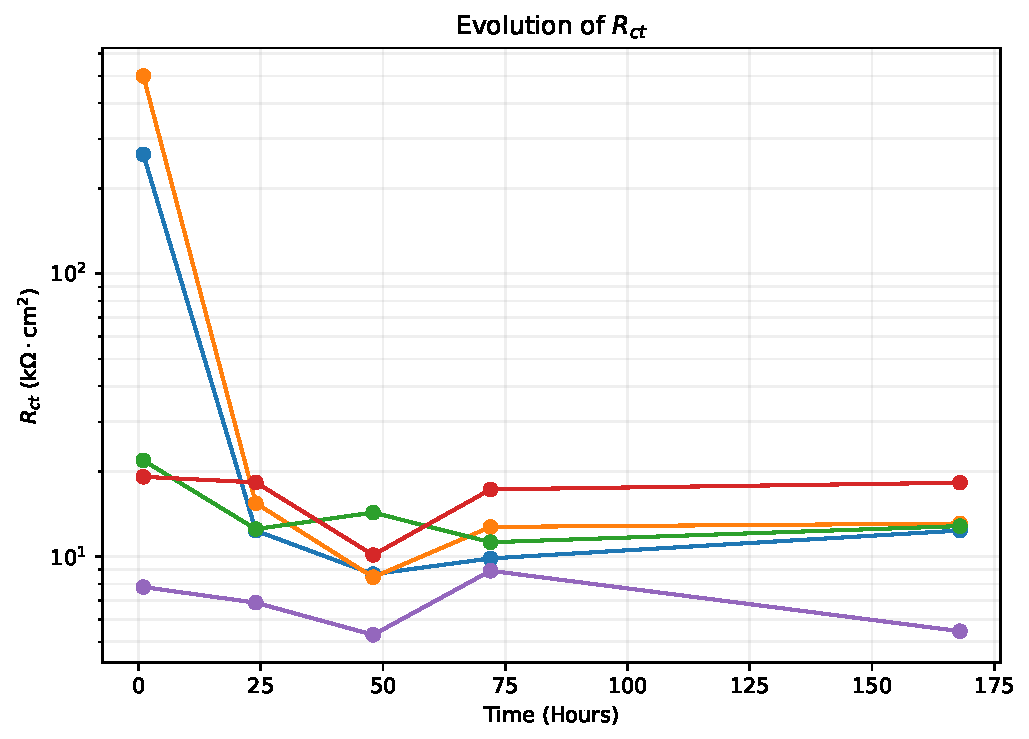
\includegraphics[width=0.9\linewidth]{Figures/Rct_evolution_LDH2_resume.pdf}
\captionof{figure}{Evolution of $R_{\text{ct}}$ over the \qty{168}{\hour} immersion period for the LDH-2 specimens.}
\label{fig:Rct_evolution_ldh2}
\end{center}

% Figure 2: Cdl Evolution
\begin{center}
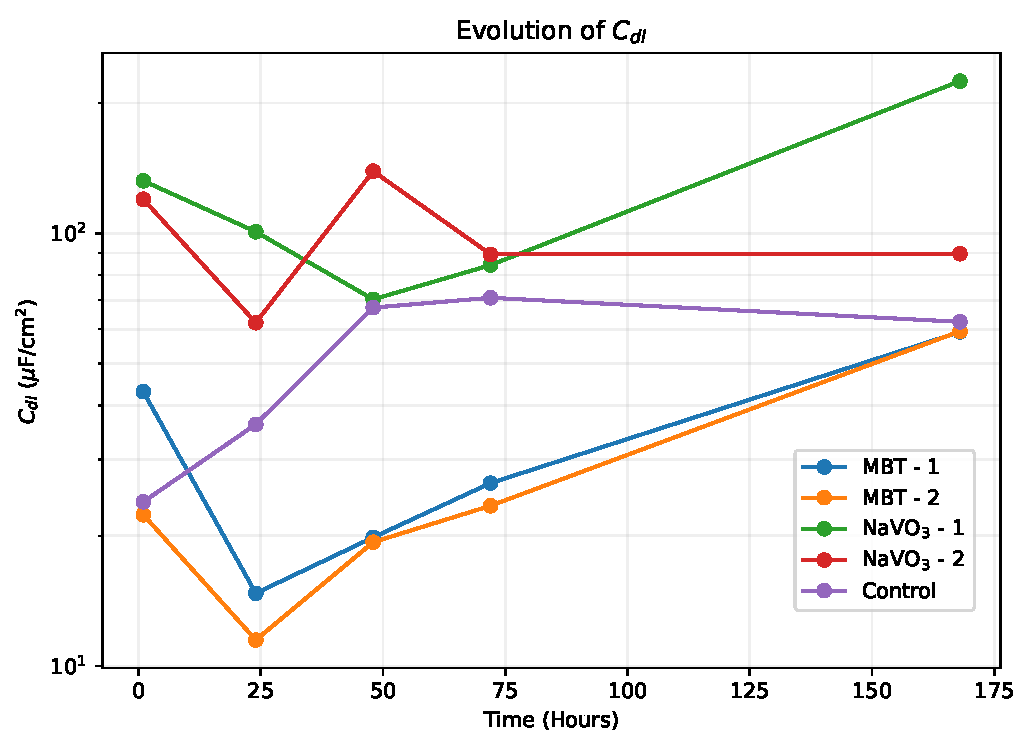
\includegraphics[width=0.9\linewidth]{Figures/Cdl_evolution_LDH2_resume.pdf}
\captionof{figure}{Evolution of $C_{\text{dl}}$ over the \qty{168}{\hour} immersion period for the LDH-2 specimens.}
\label{fig:Cdl_evolution_ldh2}
\end{center}

\subsection{Polyurethane Topcoat Application}
Finally, a polyurethane topcoat was applied to planar and complex-geometry specimens via anodic electrodeposition. Cross-sectional SEM-EDS confirmed robust interfacial adhesion and resolved the multilayer architecture, identifying the LDH layer (Zn, O) and specific intercalated species (S for MBT, V for \ce{NaVO3}). Local thickness measurements revealed a thinner coating for MBT (\qty{16.5}{\micro\meter}) compared to \ce{NaVO3} (\qty{26.5}{\micro\meter}), attributed to the amorphous remnant film versus the intact crystalline LDH. Macroscopic evaluations highlighted severe thickness inhomogeneity specifically in the MBT system, contrasting with the relatively uniform \ce{NaVO3} topcoat. Crucially, cross-sections visually confirmed the persistence of large Fe--Mn intermetallic particles at the alloy surface, highlighting the challenge of protecting these active micro-galvanic sites. Despite the MBT inhomogeneity, conformal coverage was achieved on complex geometries, validating the system's practical feasibility.


\section{Conclusions and Future Work}
This work investigated ZnAl--LDH conversion coatings on the AC46000 die-cast alloy as a chromate-free aerospace alternative. While \ce{NaVO3} was successfully intercalated and demonstrated active chloride-triggered release, MBT dissolved the LDH structure via aggressive zinc chelation. Corrosion evaluation revealed that aggressive industrial pre-treatments detrimentally exposed subsurface IMPs, whereas a milder chemical pre-treatment yielded significant improvements: MBT provided excellent initial barrier protection and \ce{NaVO3} offered sustained active protection. However, long-term performance remains limited by the inability of these inhibitors to passivate the highly prevalent Fe--Mn intermetallic particles. Ultimately, the successful conformal deposition of a polyurethane topcoat via anodic electrodeposition validated the system's practical feasibility and industrial viability for protecting complex aerospace geometries.

Future work should explore alternative inhibitors (e.g., cerium-based compounds) effective against Fe-rich phases, and alternative host compositions (e.g., MgAl--LDH) to accommodate thiol-based molecules. Long-term durability assessments via accelerated testing and localised electrochemistry (SVET, SECM), alongside mechanical benchmarking against industrial reference coatings, are required to fully validate this multilayer architecture \cite{Cao2022, Becker2019}.


{\footnotesize
\bibliographystyle{ieeetr}
\bibliography{references}
}

\end{multicols}
\end{document}